\documentclass[c,aspectratio=169]{beamer}

\graphicspath{{img/}}

\usepackage{mathspec}

\usepackage{algorithm}
\usepackage{algpseudocode}
\usepackage[ngerman]{babel}
\usepackage{changepage}
\usepackage{collect}
\usepackage{comment}
\usepackage{csquotes}
\usepackage{float}
\usepackage{hyperref}
\usepackage{listings}
\usepackage{multimedia}
\usepackage{tikz}
\usepackage[normalem]{ulem}
\usepackage[table]{xcolor}
\usepackage{siunitx}

% \setmainfont{Libertinus Serif}
% \setsansfont{Libertinus Sans}
% \setmonofont{TeX Gyre Cursor Bold}
% \setmathfont[Digits]{Libertinus Sans}

\setmainfont{Liberation Serif}
\setsansfont{Liberation Sans}
\setmonofont{Liberation Mono}
\setmathfont[Digits]{Liberation Sans}

\usetheme{Madrid}
\usecolortheme{spruce}
\setbeamercovered{invisible}
\setbeamercolor{alerted text}{fg=blue}

\setbeamertemplate{navigation symbols}{}

\usebeamercolor[bg]{palette primary}
\usebeamercolor[bg]{palette secondary}
\usebeamercolor[bg]{palette tertiary}


\newenvironment{itemblock}[1]{\begin{block}{#1}\begin{itemize}}{\end{itemize}\end{block}}
\newenvironment{withtitle}[1]{\begin{description}\item[#1]~\\}{\end{description}}

\newcommand{\todo}[1]{\colorbox{red}{\color{white}\bf TODO: #1}}
\newcommand{\dunno}[0]{\colorbox{red}{\color{white}\bf ???}}

\newcommand{\uexplain}[2]{\underbrace{\mathtt{#1}}_{\hidewidth \mathsf{#2}\hidewidth} \hskip 0.5em}
\newcommand{\oexplain}[2]{\overbrace{\mathtt{#1}}^{\hidewidth \mathsf{#2}\hidewidth} \hskip 0.5em}

\definecollection{picture-sources}

\newcommand{\sourcedimage}[5][width=\textwidth,height=0.7\textheight,keepaspectratio]{%
  \begin{center}
    \includegraphics[#1]{#2}

    \expandafter\begin{collect}{picture-sources}{}{}
      \item[#3] \href{#4}{#4} \\ #5
    \end{collect}
  \end{center}
}

\newcommand{\imageframe}[4]{%
  {
    \setbeamercolor{background canvas}{bg=black}
    \begin{frame}[plain]
        \expandafter\begin{collect}{picture-sources}{}{}
        \item[#2] \href{#3}{#3} \\ #4
        \end{collect}
        \begin{tikzpicture}[remember picture,overlay]
          \node[at=(current page.center)] {
            \includegraphics[width=\paperwidth,height=\paperheight,keepaspectratio]{#1}
          };
        \end{tikzpicture}
    \end{frame}
  }
}

\lstset{basicstyle=\ttfamily}

\renewcommand{\algorithmicforall}{\textbf{for each}}

\title[~]{\Huge Computer selbst bauen}
\subtitle{}
\author[~]{andi $\langle$andi@entropia.de$\rangle$}
\date{}

\begin{document}

{
  \setbeamercolor{background canvas}{bg=black}
  \begin{frame}[plain]
    \begin{tikzpicture}[remember picture,overlay]
      \node[at=(current page.center)] {
        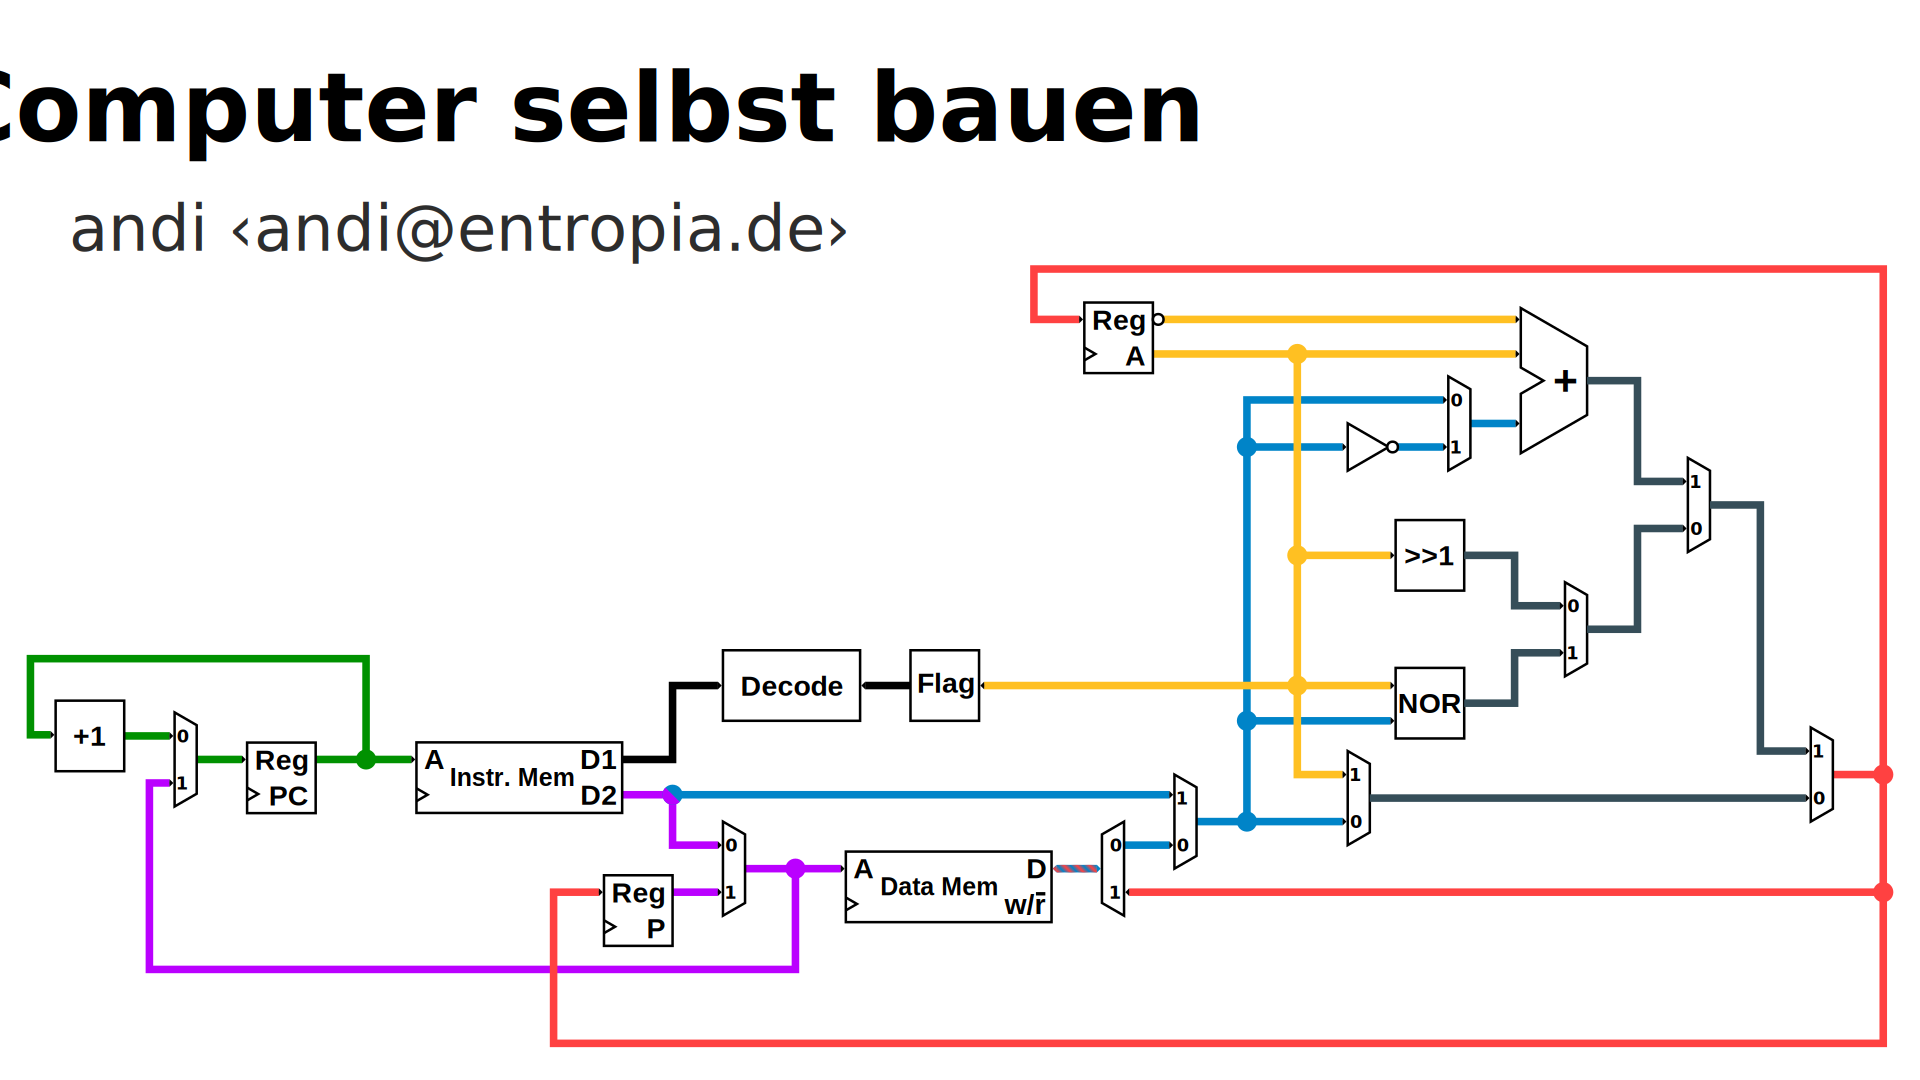
\includegraphics[width=\paperwidth,height=\paperheight,keepaspectratio]{title-slide}
      };
    \end{tikzpicture}
  \end{frame}
}

\begin{frame}
  \frametitle{Es ist kompliziert}

  \begin{columns}
    \begin{column}{.45\textwidth}
      \begin{center}
        \sourcedimage{zen2-die-shot}{Die Shot eines AMD Zen2}{https://en.wikipedia.org/wiki/File:Zen2\_Matisse\_Ryzen\_7nm\_Core\_Die\_shot.jpg}{Fritzchens Fritz, 2019. CC-0.}
        \emph{AMD Zen 2 \enquote{Matisse}}
      \end{center}
    \end{column}
    \begin{column}{.45\textwidth}
      \begin{itemize}
      \item \qty{4800000000} Transistoren
      \item Taktzeit:\\
        \qty{0.2}{\nano\second} $\hat=$ \qty{6.4} Licht-cm $\approx$ \qty{4} Strom-cm
      \end{itemize}

      \bigskip

      Mehr dazu:

      \smallskip

      \includegraphics[width=\textwidth]{talk-jadyn}
    \end{column}
  \end{columns}
\end{frame}

\begin{frame}
  \frametitle{Es geht einfacher}

  \begin{columns}
    \begin{column}{.45\textwidth}
      \sourcedimage{relay-transparent}{Transparentes Relais}{https://commons.wikimedia.org/wiki/File:Omron\_G2R-2-24V\_relay\_04.jpg}{Retired electrician, 2022. CC-0.}
    \end{column}
    \begin{column}{.45\textwidth}
      \begin{itemize}
      \item \qty{120} Relais
      \item Takt: $\approx$ \qty{1}{\second}
      \end{itemize}
    \end{column}
  \end{columns}
\end{frame}

\begin{frame}
  \frametitle{Kabel \& Gates}

  \begin{columns}
    \begin{column}{.45\textwidth}
      \hrule
    \end{column}
    \begin{column}{.45\textwidth}
      \hrule
    \end{column}
  \end{columns}
\end{frame}

\begin{frame}
  \frametitle{Busse}
\end{frame}

\begin{frame}
  \frametitle{Rechnen ist nicht schwer}

  \ldots zumindest Addieren:

  \begin{columns}
    \begin{column}{.45\textwidth}
      \begin{align*}
        0 + 0 + 0 = 00 \\
        0 + 0 + 1 = 01 \\
        0 + 1 + 0 = 01 \\
        1 + 0 + 0 = 01 \\
        1 + 1 + 0 = 10 \\
        \textcolor<2->{palette tertiary.bg}{1 + 0 + 1 = 10} \\
        0 + 1 + 1 = 10 \\
        1 + 1 + 1 = 11
      \end{align*}

      Auch nur ein Gate!
    \end{column}
    \begin{column}{.45\textwidth}
      \alt<2>{
        \begin{tabular}{ccccccccc}
          & 0 & 0 & 1 & 1 & \cellcolor{palette primary.bg}1 & 1 & 1 & 0 \\
          + & 0 & 0 & 0 & 1 & \cellcolor{palette primary.bg}0 & 1 & 0 & 1 \\
          &   &   & \scriptsize{1}  & \cellcolor{palette secondary.bg}\scriptsize{1}  & \cellcolor{palette primary.bg}\scriptsize{1}  &   &   &   \\
          \hline
          & 0 & 1 & 0 & 1 & \cellcolor{palette secondary.bg}0 & 0 & 1 & 1
        \end{tabular}
      }{
        \begin{tabular}{ccccccccc}
          & 0 & 0 & 1 & 1 & 1 & 1 & 1 & 0 \\
          + & 0 & 0 & 0 & 1 & 0 & 1 & 0 & 1 \\
          &   &   & \scriptsize{1}  & \scriptsize{1}  & \scriptsize{1}  &   &   &   \\
          \hline
          & 0 & 1 & 0 & 1 & 0 & 0 & 1 & 1
        \end{tabular}
      }

      \uncover<3>{
        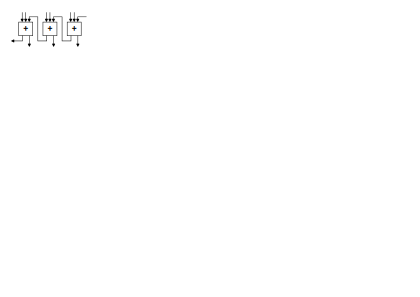
\includegraphics[width=\linewidth]{ripple-carry.pdf}
      }
    \end{column}
  \end{columns}

\end{frame}

\begin{frame}
  \frametitle{\ldots und fertig ist der ASIC}

  \begin{columns}
    \begin{column}{.45\textwidth}
      \begin{center}
        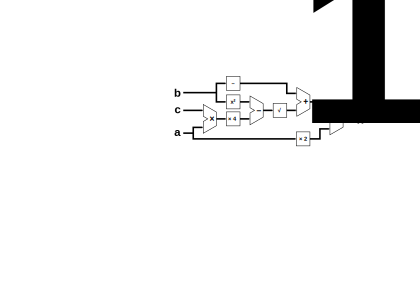
\includegraphics[width=\linewidth]{abc-formel.pdf}

        \[ x_1 = \frac{-b + \sqrt{b^2 - 4ac}}{2a} \]
      \end{center}
    \end{column}
    \begin{column}{.45\textwidth}
      Was fehlt?
      \begin{itemize}
      \item Auswahl
      \item Speicher
      \item Programm
      \end{itemize}
    \end{column}
  \end{columns}
\end{frame}

\begin{frame}
  \frametitle{Auswahl}

  Wichtigstes Modul: \textbf{Multiplexer}
\end{frame}

%% 1. aussuchen, was machen
%% 2. mehrere dinge hintereinander

%% MUX

%% ALU

%%




\begin{frame}
  \frametitle{Bildnachweis}
  \tiny
  \begin{description}
    \includecollection{picture-sources}
  \end{description}
\end{frame}

\end{document}